\documentclass{article}

\usepackage[margin=1in]{geometry}
\usepackage{setspace}
\usepackage{graphicx}

\title{Final Project - Status Update 2}
\author{Michael Forney \\ SID: 21392560}

\begin{document}
    \maketitle
    \doublespacing

    My implementation of a variation on the cyclic coordinate decent inverse
    kinematics algorithm is now working correctly. It works very quickly for
    constraints near the end of the arm, but joint structures where a lower
    node is constrained as well converge more slowly because the joint does not
    want to disrupt the ends which often have already converged. I plan to
    solve this problem by doing CCD first on the constraints closer to the root
    node, and then gradually working my way to the ends.

    I have implemented a mechanism to select, and display information about a
    node, but am still working on allowing the user to manually configure a
    joint by dragging it around. Also, I need to add a timeline tab to the
    lower bar to allow the user to insert poses to generate an animation. I am
    pretty confident I will be able to get this done in the next week.

    Here are some screenshots of my program working:

    \begin{center}
        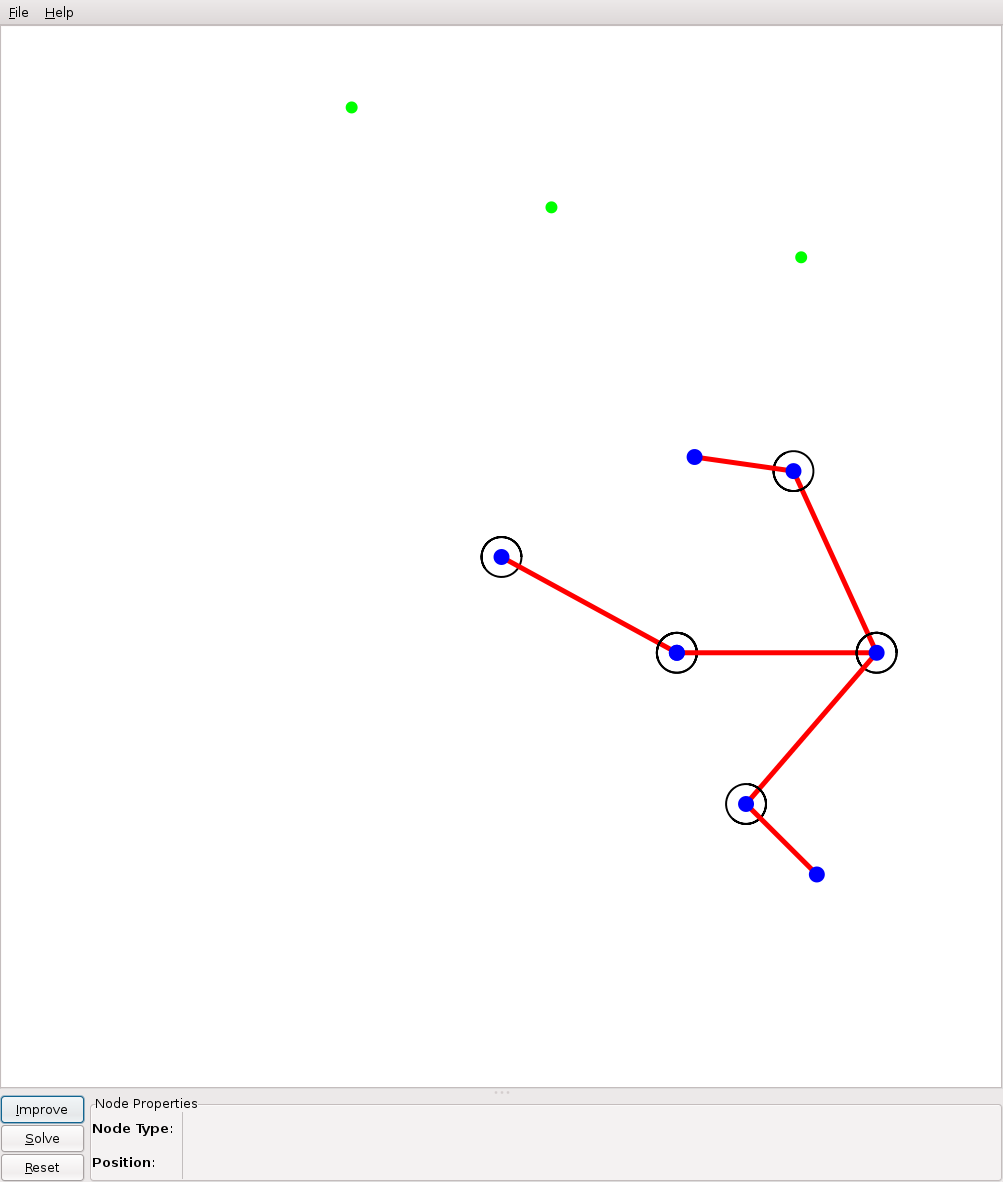
\includegraphics[width=400px]{pose_1.png} \\
        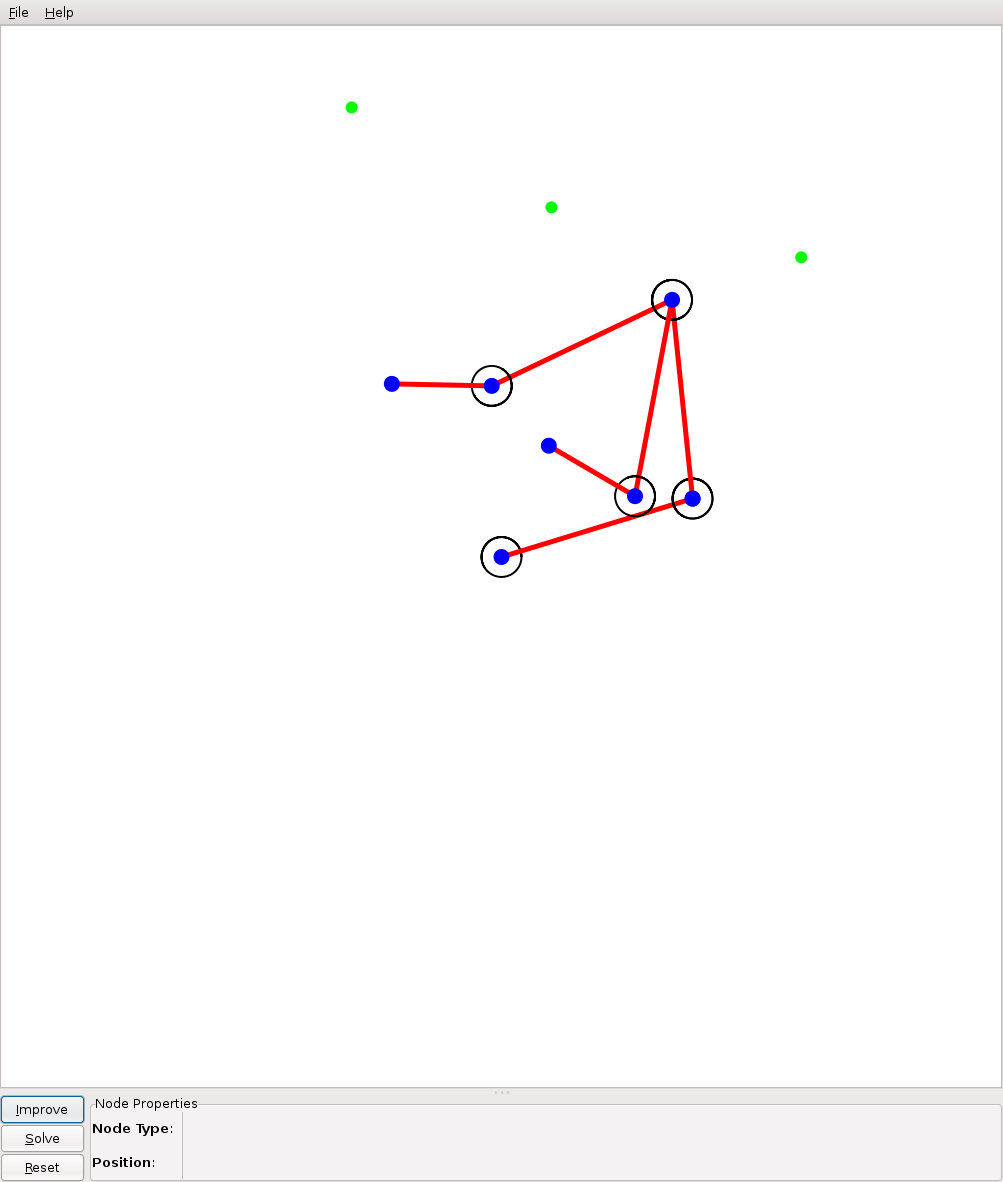
\includegraphics[width=400px]{pose_2.png} \\
        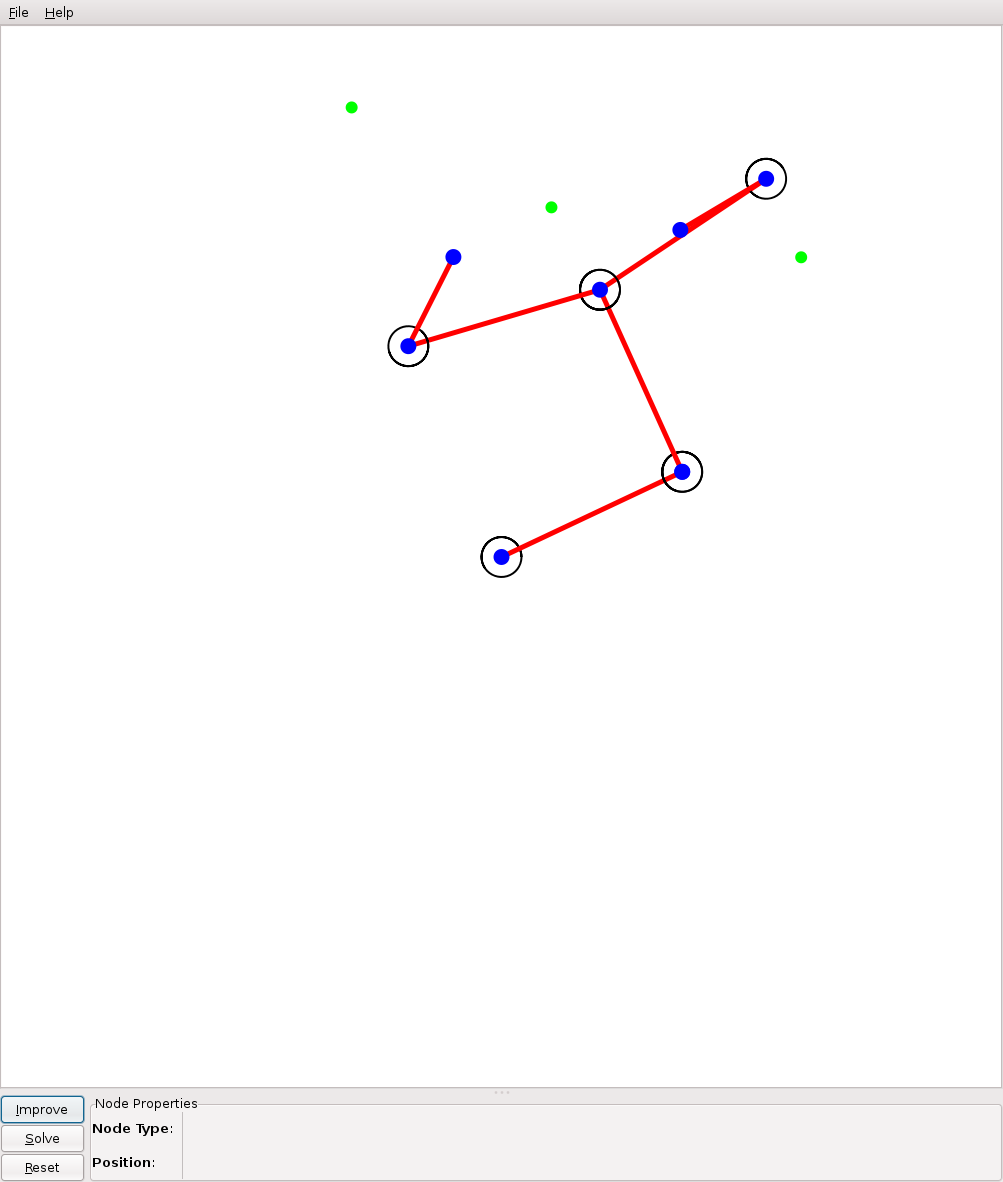
\includegraphics[width=400px]{pose_3.png} \\
        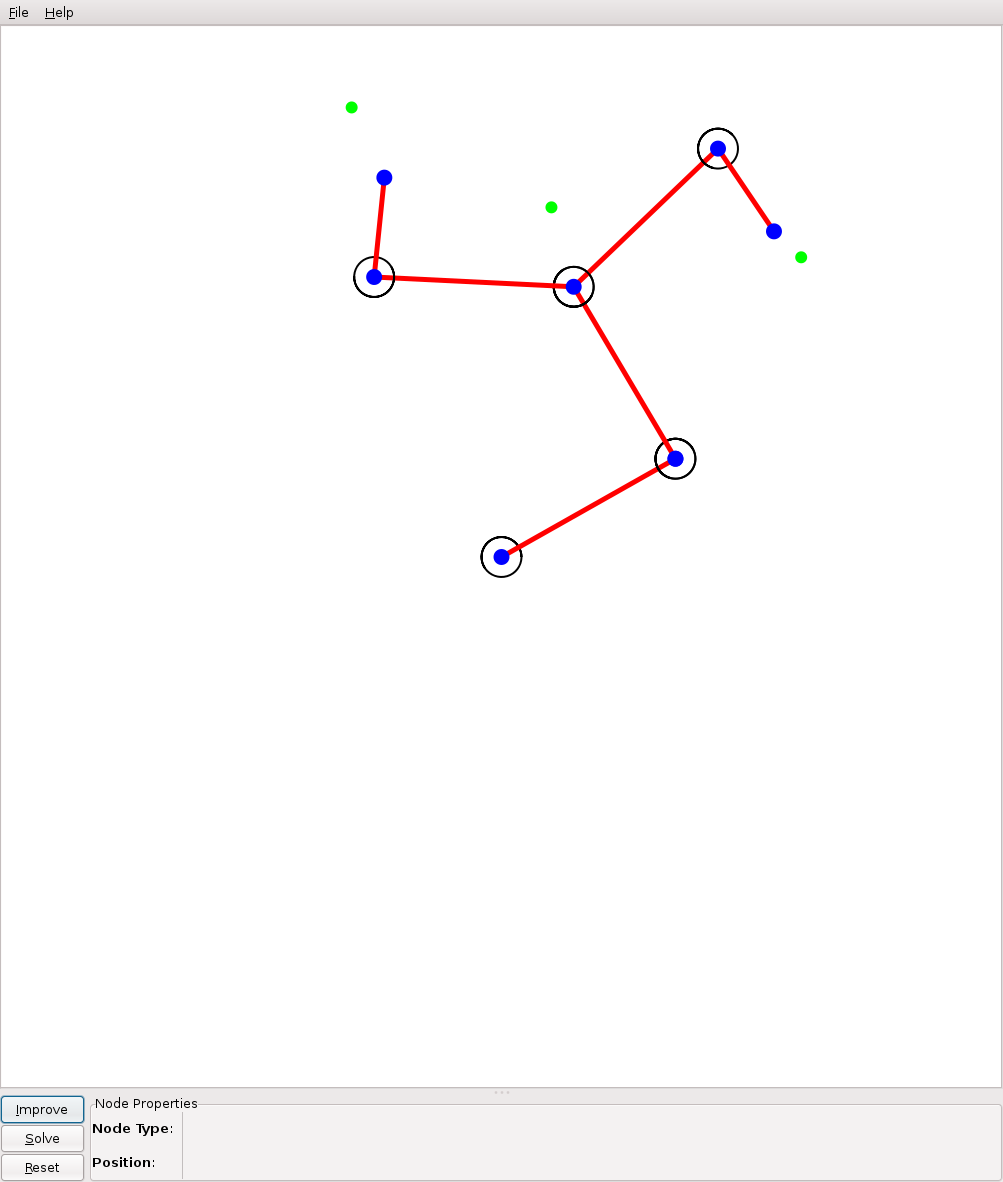
\includegraphics[width=400px]{pose_4.png} \\
        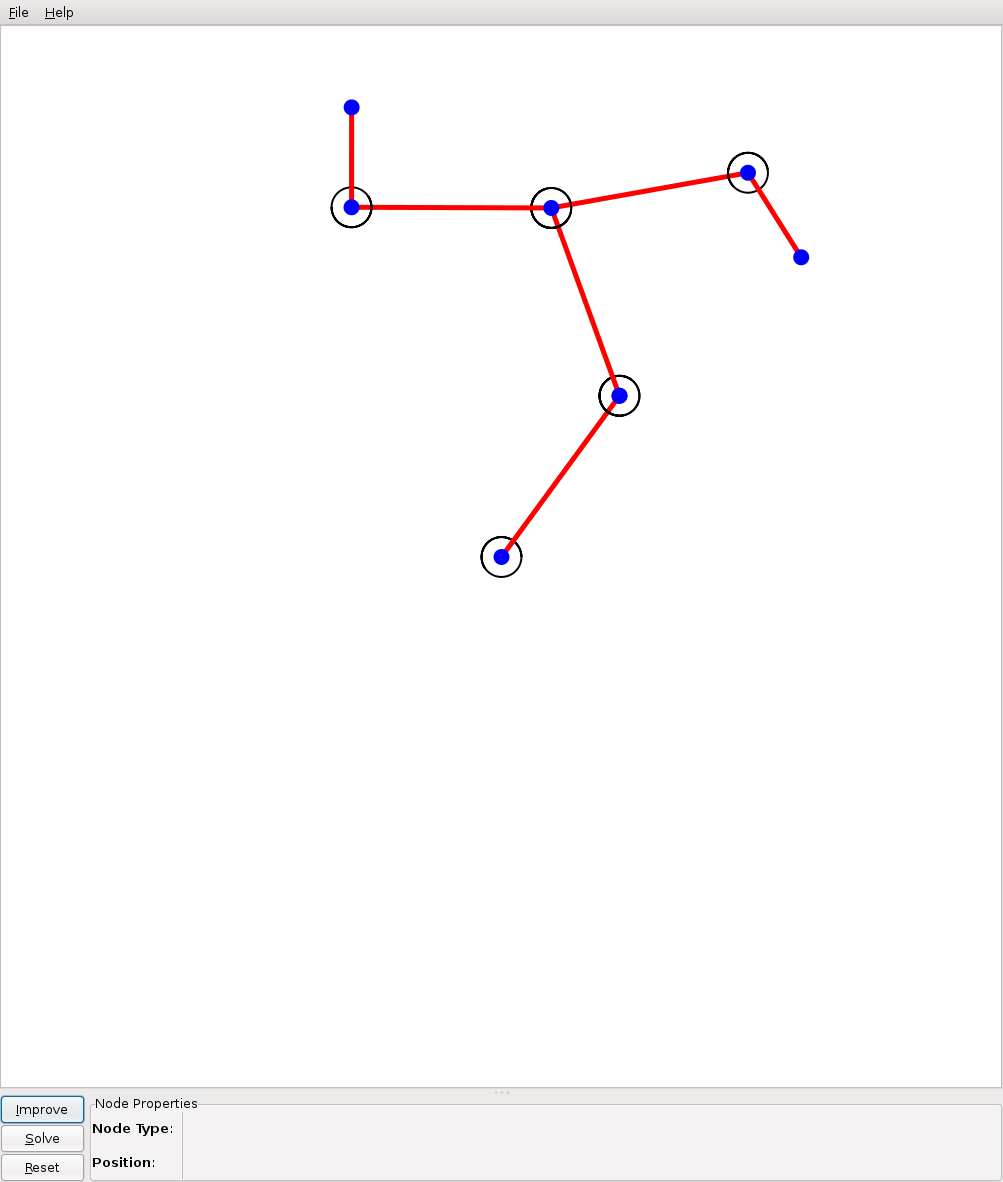
\includegraphics[width=400px]{pose_final.png}
    \end{center}

\end{document}

